
\documentclass[../draft_1.tex]{subfiles}

\begin{document}

\chapter{Implementation and Numerical Results}

\section{Discretisation Scheme}
In this chapter we will look at how the \textit{solver} we derived actually performs in some test cases. We looked at problems with a one-dimensional space domain $\mathcal{S} = (0, S)$ and a time-interval $\mathcal{T} = (0,T)$, that is 
\begin{ceqn}
\begin{equation}
\Omega = (0, S) \times (0, T), \quad S,T > 0
\end{equation}
\end{ceqn}
and which we discretised using uniformly-sized rectangular elements. Let $N_x$ be the number of elements in space and $N_t$ the number of elements in time. As a finite-dimensional approximation space we used piecewise linear polynomials in space and time for the approximation of $\sigma_h$ as well as $u_h$ and chose the local basis \\

\begin{minipage}[l]{0.5\linewidth}
	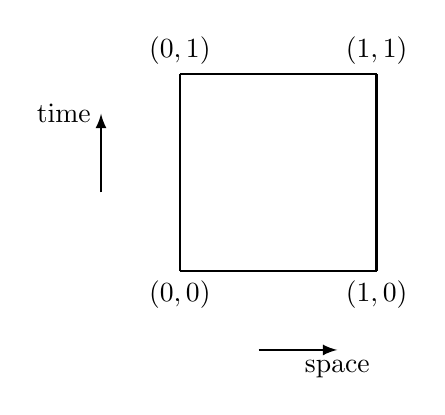
\begin{tikzpicture}
	% Draw the grid
	\tikzset{help lines/.style={color=black}}
	\draw[thick,step=2.5cm] (0,0) grid (2.5,2.5);
	

	 \node [anchor=north] at (0,0) {$(0,0)$};
	 \node [anchor=north] at (2.5,0) {$(1,0)$};
	 \node [anchor=south] at (0,2.5) {$(0,1)$};
	 \node [anchor=south] at (2.5,2.5) {$(1,1)$};
	 
	 
	 \draw[thick,-latex] (1,-1) -- (2,-1) node[below] {space};
	 \draw[thick,-latex] (-1,1) -- (-1,2) node[left]{time};
	 
	\end{tikzpicture}
	
\end{minipage}% 
\begin{minipage}[r]{0.5\linewidth}
\begin{ceqn}
	\begin{equation}
	\begin{aligned}
	\phi_{11}(x,t) &= (1- x) &\cdot (1-t) \\
	\phi_{12}(x,t) &=  x  &\cdot  (1-t) \\
	\phi_{21}(x,t) &= (1- x) &\cdot t  \\
	\phi_{22}(x,t) &= x  &\cdot  t 
	\end{aligned}
	\end{equation}
	\end{ceqn}
\end{minipage}

If we translate this from local to the global coordinates and scale appropriately according to the mesh size with an appropriate projection, we have that 
\begin{ceqn}
	\begin{equation}
	\begin{aligned}
	\phi_{ij}(x_k, t_l) = \begin{cases} 1 \quad \text{if } (k,l) = (i,j)  \\ 0 \quad \text{otherwise} \end{cases}
	\end{aligned}
	\end{equation}
	\end{ceqn}

We arrange the grid points the same way the local basis is labeled, that is for a fixed $t_j$ all elements in space with $x_i < x_{i+1}$, and subsequently all space elements for $t_{j+1}$. As previously mentioned the we arranged $\sigma_h$ and $u_h$ such that they are two concatenated vectors. Hence one obtains a system of equations with $m = (N_x + 1 )\cdot (N_t + 1)$ degrees of freedom for $\sigma_h$ and the same again for $u_h$. The solution vector is therefore of $2m$ while the matrices have a size of $2m \times 2m$. It is possible to use this local basis for $\sigma_h$ and $u_h$ because we are in the one-dimensional case and therefore $ \nabla u = \partial_x u = \sigma$ and $div(\sigma) = \partial_{x} \sigma$. For $dim (\mathcal{S}) > 1 $ we would have to treat this problem differently using for example Raviart-Thomas elements [source], which is however beyond the scope of this thesis \textit{but could be of interest in future investigations}. In order to compute the individual integral terms we used a quadrature rule of degree three, that is we get the exact integral for the linear apprximations of the functions. The admissible boundary conditions are a mixture of Dirichlet and Neumann type and are directly imposed in the system, either in $u$ or $\sigma$, respectively. 

\section{Multigrid Implementation}
We implemented a geometric multigrid V-cycle, where the number of elements on the coarse grid and the number of levels are chosen and then all other grids, interpolation operators, and finer level operators are generated automatically. The reason behind this is to guarantee nested meshes. As discussed previously there is no unique best problem indepedent coarsening strategy, and especially in the case of space-time discretisations it has a great effect on the overall performance. Unfortunately the literature on what could be a favourable strategy in a least squares space-time set up was very sparse and therefore we decided to use a classical space-time coarsening approach, where the size of each rectangle grows by a factor of 4 with each coarsening because the length of the element is doubles in each direction, see figure [...] below. It means that with each coarsening step the number of elements reducs by a factor of $(2^{-2})$ and therefore also the degrees of freedom. This seemed like a reasonable approach, since we are dealing with a coupled first order system, and hence considerations like in \cite{gander2016analysis}, that \textit{showed} it would to be preferrable to keep the quotient $\lambda = \frac{d \Delta t}{\Delta x^2}$ (where $d$ decribes the diffusion constant and $\Delta t$ and $\Delta x$ the respective step sizes) close to one on all levels, did not really apply here because we have no second order derivative, that would lead to the square term in space. So under the assumption that the diffusion term $d$ is not too different from one and we choose a similar stepsize in space and time, the standard space-time coarsening would lead to a coefficient that is the same on all levels as well as close to one. More extensive testing on this beyond the scope of this thesis. \textit{Rough estimates showed that for the linear case this seemed to be the case as a interpolation operators of type \cite{gander2016analysis} seemed to lead to slower convergence.} 
\smallskip
\\
We then chose to use interpolation weights according to the following scheme, where fuilled dots represent coarse grid points and the blank circles fine grid points \\

\begin{minipage}[l]{0.5\linewidth}
	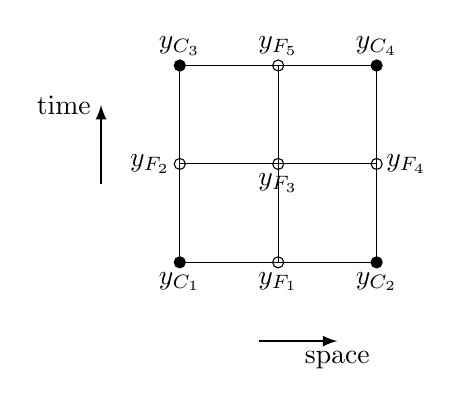
\begin{tikzpicture}
	% Draw the grid
	\tikzset{help lines/.style={color=black}}
	\draw[thin,step=1.25cm, help lines] (0,0) grid (2.5,2.5); 
	

    \draw[black, fill=black] (0,0) circle(2pt);
    \draw[black, fill=black] (2.5,0) circle(2pt);
    \draw[black, fill=black] (0,2.5) circle(2pt);
    \draw[black, fill=black] (2.5,2.5) circle(2pt);
    
    \draw[black] (1.25,0) circle(2pt);
    \draw[black] (0,1.25) circle(2pt);
    \draw[black] (1.25,1.25) circle(2pt);
    \draw[black] (2.5,1.25) circle(2pt);
    \draw[black] (1.25, 2.5) circle(2pt);
    
	 \draw[thick,-latex] (1,-1) -- (2,-1) node[below] {space};
	\draw[thick,-latex] (-1,1) -- (-1,2) node[left]{time};
	
	\node [anchor=north] at (0,0) {$y_{\text{C}_1}$};
	\node [anchor=north] at (2.5,0) {$y_{\text{C}_2}$};
	\node [anchor=south] at (0,2.5) {$y_{\text{C}_3}$};
	\node [anchor=south] at (2.5,2.5) {$y_{\text{C}_4}$};
	
	\node [anchor=north] at (1.25,0) {$y_{\text{F}_1}$};
	\node [anchor=east] at (0,1.25) {$y_{\text{F}_2}$};
	\node [anchor=north] at (1.25,1.25) {$y_{\text{F}_3}$};
	\node [anchor=west] at (2.5,1.25)  {$y_{\text{F}_4}$};
	\node [anchor=south] at (1.25,2.5) {$y_{\text{F}_5}$};
	
	\end{tikzpicture}
	

\end{minipage}%
\begin{minipage}[r]{0.5\linewidth}
\begin{ceqn}
	\begin{equation}
	\begin{aligned}
	s(y_{\text{C}_i})  &= s(y_{\text{C}_i})  \qquad \forall i \\	
	s(y_{\text{F}_1}) &= \frac{1}{2} y_{\text{C}_1} + \frac{1}{2} y_{\text{C}_2} \\
	s(y_{\text{F}_2}) &= \frac{1}{2} y_{\text{C}_1} + \frac{1}{2} y_{\text{C}_3} \\
	s(y_{\text{F}_3}) &= \frac{1}{4} y_{\text{C}_1} + \frac{1}{4} y_{\text{C}_2} + \frac{1}{4} y_{\text{C}_3} + \frac{1}{4} y_{\text{C}_4} \\		
	s(y_{\text{F}_4}) &= \frac{1}{2} y_{\text{C}_2} + \frac{1}{2} y_{\text{C}_4} \\
	s(y_{\text{F}_5}) &= \frac{1}{2} y_{\text{C}_3} + \frac{1}{2} y_{\text{C}_4} \\
	\end{aligned}
	\end{equation}
	\end{ceqn}
\\
\end{minipage}

They are constructed respectively to go recursively from one level to the next, and this is for either $\sigma_h$ or $u_h$. If $\tilde{I}$ is an interpolation matrix of the above type then we will have that the overall interpolation operator will have the following form, that is we interpolate independently for the two variables. 
\begin{ceqn}
	\begin{equation}
	I = \begin{bmatrix}
	\tilde{I} & 0 \\
	0 & 	\tilde{I}
	\end{bmatrix}
	\end{equation}
\end{ceqn}

The interpolation matrix from level $k-1$ to level $k$ is as before denoted by $I_{k-1}^k$ and we have that  $I_{k-1}^k \in \mathbb{R}^{2m_k \times 2m_{k-1}}$, where $m_k$ and $m_{k-1}$ denotes the number of points on the space time grid on the respective level. 

\begin{figure}[ht!]
	\centering
	\includegraphics[scale=0.25]{images/implementation/sol_heat_eqn_interpol}
	\caption{Interpolation of the solution to the heat equation with $u(x,0) = \max(1-2x, 0)$, $D(x) = 0.1$ and homogeneous Neumann boundary conditions in time on a unit square from $8 \times 8$ to $16 \times 16$ elements. The interpolated solution of $\sigma$ is not shown here as $\tilde{I}$ simply applied to $\sigma$ and $u$ independently.}
\end{figure}

Visually the function on the right really appears to be a good interpolation of the function on the left, transmitting \textit{global} information. \textit{In the multigrid implementation we remove the influence of the boundary conditions.}

\subsection{Smoothers}
Smoothers are a key part of an efficient multigrid algorithm. And while many of them may theoretically be a possibility, in practice the choice of a suitable smoother is often not an easy one. We would like that the combination of coarse grid correction and smoother reduces the error efficiently for all frequencies. In the case of a geometric multigrid applied to an elliptic problem the coarse grid correction captures the low frequency error quickly while most smoothers like (block-) Jacobi or Gauss-Seidel reduce the high frequency error well and therefore the two are a favourable synthesis. But as we are also trying to develop a highly parallelisable solver it is of course important to also be taking that into account when choosing a smoother, therefore a regular Gauss-Seidel iteration is for example not a suitable choice as it works sequentially. In our set up we also have the additional feature of the two coupled variables $\sigma_h$ and $u_h$, which are separated in the sense that they are two concatenated vectors but have the contentual connection. Therefore it might be favorable to use a (block-) smoother that takes this relationship into account. Hence we decided to use a Vanka type [source?] block Jacobi relaxation. That is a block Jacobi smoother where each block contains all degrees of freedom associated to one grid point in the space-time domain. That is we choose rectangular patches of size $p \times q$ on the domain, that is $p$ points in space and $q$ in time, construct a submatrix containing all entries of $A$ associated to those nodes for $\sigma_h$ and $u_h$ and all of the corresponding coupling terms and directly invert the small submatrix. We partition the entire domain like that, while potentially having smaller patches on the boundary, and finally assemble a preconditioner $P$ containing the inverted submatrices. Due to the organisation of $\sigma_h$ and $u_h$, $P$ will not be a block diagonal matrix. For $p = q = 2 $ we would have the following patches, where $\tilde{c}_i$ describes the set of indices assosciated with the patch, and $C_i$ the corresponding submatrix, which are each of size $8 \times 8$. 

\begin{figure}[ht!]
	\centering
	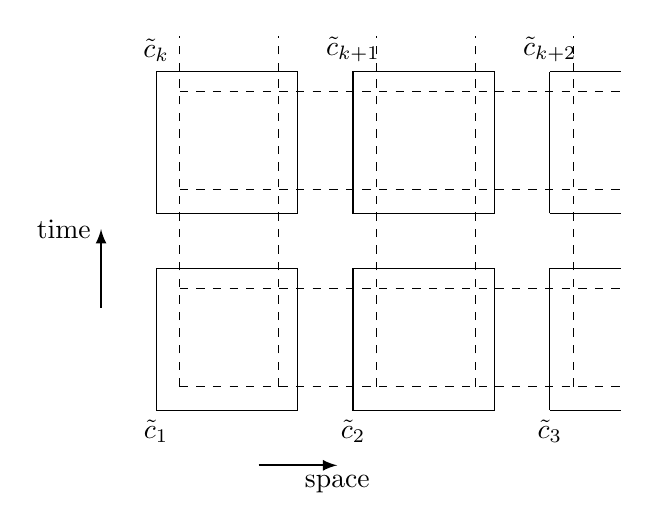
\begin{tikzpicture}
	% Draw the grid
	\tikzset{help lines/.style={color=black, dashed}}
	\draw[thin,step=1.25cm, help lines] (0,0) grid (5.6,4.45); 
	
	\draw[thick,-latex] (1,-1) -- (2,-1) node[below] {space};
	\draw[thick,-latex] (-1,1) -- (-1,2) node[left]{time};
	
	\draw[black] (-0.3,-0.3) rectangle  (1.5,1.5);
	\draw[black] (2.2,-0.3) rectangle  (4,1.5);
	
	\draw[black] (-0.3,2.2) rectangle  (1.5,4);
	\draw[black] (2.2,2.2) rectangle  (4,4);
	
	\draw[black] (4.7, -0.3) -- (5.6,-0.3);
	\draw[black] (4.7, -0.3) -- (4.7, 1.5);
	\draw[black] (4.7, 1.5) -- (5.6,1.5);	
	
	\draw[black] (4.7, 2.2) -- (5.6,2.2);
	\draw[black] (4.7, 2.2) -- (4.7, 4);
	\draw[black] (4.7, 4) -- (5.6,4);	
	
	\node [anchor=north] at (-0.3,-0.3) {$\tilde{c}_1$};
	\node [anchor=north] at (2.2, -0.3) {$\tilde{c}_2$};
	\node [anchor=north] at (4.7, -0.3) {$\tilde{c}_3$};	
	
	\node [anchor=south] at (-0.3,4) {$\tilde{c}_k$};
	\node [anchor=south] at (2.2, 4) {$\tilde{c}_{k+1}$};
	\node [anchor=south] at (4.7, 4) {$\tilde{c}_{k+2}$};		
	\end{tikzpicture}
	\caption{Schematic overview of the construction of the blocks of damped Jacobi smoother}
\end{figure}

\textit{damped Jacobi} \\
Below we can see how the smoother acts on a random initial guess for the linear system $As = f$, where $A$ is the least squares finite element matrix arising from the functional $J([\sigma, u], 0)$ with the discretisation chosen as described in chapter 4 and the previous parts of this chapter, and $f$ is a zero right-hand side that only contains the boundary conditions. That is we look at the iteration 
\begin{ceqn}
	\begin{equation}
	e_{k+1} = e_k + \omega P (f - Ae_k)
	\end{equation}
\end{ceqn}
where $P$ is the preconditioner and $\omega$ stands for the damping factor. Since we have a zero forcing term, the exact solution is zero everywhere if we have homogenous boundary conditions, and hence $e_k$ describes the remaining error in each iteration starting from an initial guess. 

% for contourplot 1 it took 8184 iterations to have residual <10^(-9)

\begin{figure}[ht!]
	\centering
	\includegraphics[scale=0.28]{images/implementation/contour_plot_1_blk_size1by1}
	\caption{Iterates after $k = 0,3,8, 20$ iterations for a patch size of $1 \times 1$, and a grid with $11 \times 11$ elements. needed more than 9000 iterations in order for the norm of the residual to be $< 10^{-9}$.}
\end{figure}

We can see that the damped block Jacobi smoother really leads to a fast reduction of the high frequency error whereas the low frequency error is only reduced very slowly. \textit{something about computationally very cheap.} Again we only plotted $u$ as $\sigma$ behaves in the same way, simply with different boundary conditions. 

\begin{figure}[ht!]
	\centering
	\includegraphics[scale=0.28]{images/implementation/contour_plot_1_blk_size3by4}
	\caption{Iterates after $k = 0,3,8, 20$ iterations for a patch size of $3 \times 4$, and a grid with $11 \times 11$ elements. needed more than 3177 iterations in order for the norm of the residual to be $< 10^{-9}$.}
\end{figure}

Another type of smoother that we tested is a Gauss-Seidel \textit{line smoother} \cite{adams2001distributed} which can also be categorised as a Vanka smoother  \textit{write more about that reference?}. One considers each spatial degree of freedom individually but together for all times as well as the values for $\sigma$ and $u$. We extract all matrix values for each of the $x_i$, to construct submatrices. We then first solve exactly for all odd subsets of $\tilde{c}_i$, here coloured in black and update the solution before solving for all even subsets, here coloured in red. Hence for all subsets labeled in black we can solve in parallel, and subsequently for all subsets in red. 

\begin{figure}[ht!]
	\centering
	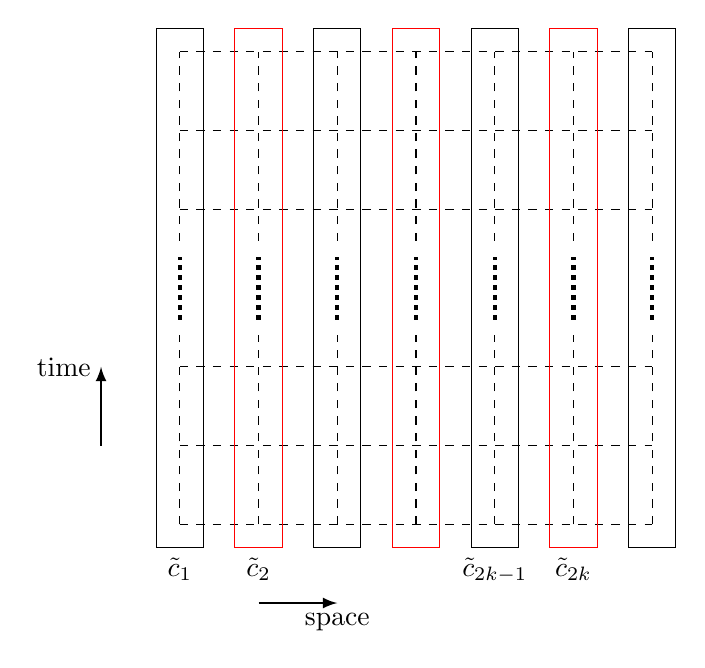
\begin{tikzpicture}
	% Draw the grid
	\tikzset{help lines/.style={color=black, dashed}}
	\draw[thin,step=1cm, help lines] (0,0) grid (6,2.4); 	
	\draw[thin,step=1cm, help lines] (0,3.6) grid (6,6); 
	
	\draw [black, dotted, ultra thick] (0, 2.6) -- (0, 3.4);
	\draw [black, dotted, ultra thick] (1, 2.6) -- (1, 3.4);
	\draw [black, dotted, ultra thick] (2, 2.6) -- (2, 3.4);
	 \draw [black, dotted, ultra thick] (3, 2.6) -- (3, 3.4);
	 \draw [black, dotted, ultra thick] (4, 2.6) -- (4, 3.4);
	\draw [black, dotted, ultra thick] (5, 2.6) -- (5, 3.4);
	\draw [black, dotted, ultra thick] (6, 2.6) -- (6, 3.4);		  
		  
	\draw[thick,-latex] (1,-1) -- (2,-1) node[below] {space};
	\draw[thick,-latex] (-1,1) -- (-1,2) node[left]{time};
	
	\draw[black] (-0.3,-0.3) rectangle  (0.3,6.3);
	\draw[red] (0.7,-0.3) rectangle  (1.3,6.3);
	\draw[black] (1.7,-0.3) rectangle  (2.3,6.3);
	\draw[red] (2.7,-0.3) rectangle  (3.3,6.3);
	\draw[black] (3.7,-0.3) rectangle  (4.3,6.3);
	\draw[red] (4.7,-0.3) rectangle  (5.3,6.3);
	\draw[black] (5.7,-0.3) rectangle  (6.3,6.3);	
	
	\node [anchor=north] at (0,-0.3) {$\tilde{c}_1$};
	\node [anchor=north] at (1, -0.3) {$\tilde{c}_2$};
	
	\node [anchor=north] at (4, -0.3) {$\tilde{c}_{2k-1}$};	
	\node [anchor=north] at (5, -0.3) {$\tilde{c}_{2k}$};					
	
	\end{tikzpicture}
	\caption{Schematic overview of the construction blocks in the Gauss Seidel line smoother}
\end{figure}

We repeated the same test as before where the preconditioner $P$ is now defined by the above description. 

\begin{figure}[ht!]
	\centering
	\includegraphics[scale=0.28]{images/implementation/contour_plot_1_lineSm}
	\caption{Iterates after $k = 0,3,8, 20$ iterations for the described line smoother, using a grid with $11 \times 11$ elements. It needed more than about 1759 iterations in order for the norm of the residual to be $< 10^{-9}$. where $A, f$ as before}
\end{figure}

As one might expect the line smoother converges much faster than the block Jacobi iteration, since the individual blocks we solve for exactly are larger. We can also see that the regions become more homogenous more quickly. \textit{there are quite large areas where we go below 0, why?}. But obviously this comes with an increase in the computational cost. 
\\
Performs much better than 3 by 4, why? Gauss Seidel? 

\pagebreak
\section{Numerical Test Cases}
\subsection{Heat Equation}

After having discussed the individual multigrid terms let us look at the overall multigrid performance for a heat equation using the derived LSFEM space-time discretisation. 
\bigskip
\\
\textit{parameters, boundary conditions, grid sizes, ...}
\bigskip
\\
\textit{pictures, this is how the solution looks like}
\bigskip
\\
\textit{some tables with convergence results}
also how many steps do we need until convergence of the smoothers by itself
\bigskip
\\
\textit{further analysis? test laplace and $u_t$ independently, what can we see from there?}
\\
\textit{Galerkin not Galerkin assembly, try with both}


% do analysis of coarse grid correction
 for the particular problem one is looking 
% how to divide sections? 
% block Jacobi, write different version
% analyse difference, error doesnt seem smooth in space, but can't really see it when looking at solution ... 

\subsection{Linearisation of a Monodomain Equation}

Before considering the full nonlinear problem we draw our attention to its linearisation in a neighbourhood of the solution $s$, the full description of how to obtain this solution we refer to the next section. Under the assumption that we have a unique local minimiser of the problem, we know that we have convexity close to the solution, that is the hessian $H_s = H(s)$ is positive definite and the gradient is very close to zero. \\
In order to better understand the behavior of the hessian around the solution we perform an error analysis using a Jacobi smoother on the linearised system. More specifically we want to see how small pertubations in the solution in areas of the wavefront and the constant regions behave under the iteration of the smoother. \textit{This could be in order to construct adapted coarse spaces that take these different local behaviors into account.} \\
We consider the following iteration 
\begin{ceqn}
	\begin{equation}
	\begin{aligned}
e_{k+1} &= e_k + P(\nabla J - H_s e_k) \quad \text{ or} \\
e_{k+1} &= e_k - P H_s e_k 
	\end{aligned}
	\end{equation}
\end{ceqn}
if we assume exactly that $\nabla J = 0$, and where $P$ describes the preconditioner. We now let $e_0$ equal to zero except for a small pertubation either in the area of the wavefront or the constant regions and see how this behaves under iteration.

\begin{ceqn}
	\begin{equation}
	\begin{aligned}
u_{k+1} &= u_k - H_k^{-1}(\nabla J_k) \\
H_k u_{k+1} &= H_k u_k - \nabla J_k, \\ 
\\
\text{ let } r_k := H_k u_k - \nabla J_k
\text{ and solve } H_k u_{k+1} = r_k \quad \text{using multigrid}
	\end{aligned}
	\end{equation}
\end{ceqn}



\subsection{Monodomain Equation}

The simplified monodomain equation that shows the movement of an excitation front through space-time looks as follows

\begin{ceqn}
	\begin{equation}
	\begin{aligned}
\partial_t u - div(D \nabla u) &= u (1 - u ) (\alpha - u), \qquad &D > 0, \ 0 < \alpha < 1 \\
u(x, 0) &= u_0(x) &\forall \ x \in S \\
\nabla u \cdot n &= 0 \qquad &\forall \ (x,t) \in \{ x \in \{0,S\}, t \in (0,T) \} 
	\end{aligned}
		\end{equation}
\end{ceqn}
We can see that the right-hand side is clearly nonlinear as it describes a third order polynomial. It can be shown that the equation has 3 fixed points, two stable fixed in zero and one, and an unstable fixed point in $\alpha$ \cite{deuflhard2011adaptive}. Hence depending on the initial conditions $u_0$ the solution will tend to either zero or one, unless it is exactly $\alpha$ and then through diffusion, very much dependent on diffusion constant though, if there is values larger than $\alpha$ eventually lead to an activation of entire domain. Below we can see approximations of the solution.

talk about non convexity, therefore using a direct solver \\
Show what solution looks like, wavefront with initial conditions \\
we can clearly see that this is only the excitation and not the depolarisation, (is maybe less of an interest as long as is it depolarises again eventually)
\begin{figure}[ht!]
	\centering
	\includegraphics[scale=0.3]{images/implementation/sol_d0_001_1by20_20by40elem}
	\includegraphics[scale=0.3]{images/implementation/sol_d0_003_1by20_20by40elem}
	\caption{For both graphs we have $u_0 = max(1-2x, 0)$, homogeneous Neumann boundary conditions on the spatial boundaries of the domain, for 20 elements in space and 40 in time. On the left we have a diffusion constant $D= 10^{-3}$, whereas on the right we have $D=3 \cdot 10^{-3}$.}
\end{figure}
The two equations giving rise to the above solutions only differ in the choice of the diffusion constant $D$. As to be expected we can see that with a larger value of $D$, the activation happens much more quickly. We can also see that the front is not as steep, as we have a faster transport of electric potential through space. 
\smallskip
\\
As previously mentioned the solutions are obtained using a dogleg trust region method for the nonlinear iteration, which is a combination of a gradient descent and a Newton iteration. \textit{More specifically we have ... description of the algorithm. ONLY WORKS FOR LOCALLY POS DEF.....	which we have. WHY NOT NEWTON UNLESS NOT SPD THEN GRADIENT DESCENT, maybe i can check for convexity in a point and if not just do gradient descent?!!} 	
\smallskip
\\
We are using a quadratic model to approximate the functional $J$, that is we solve

\begin{ceqn}
	\begin{equation}
	\begin{aligned}
\min_p m(p) = f + g^T p + \frac{1}{2} p^T H p \qquad s.t. \ ||p|| \leq \Delta, \ p \in span\{g, H^{-1}g\}. 
	\end{aligned}
	\end{equation}
\end{ceqn}

\begin{ceqn}
	\begin{equation}
	\begin{aligned}
p^U = - \frac{g^Tg}{g^T H g} g
	\end{aligned}
	\end{equation}
\end{ceqn}

\begin{ceqn}
	\begin{equation}
	\begin{aligned}
	\tilde{p}(\tau) = \begin{cases}
	\tau p^U \qquad &0 \leq \tau \leq 1 \\
	p^U + (\tau - 1)(p^B - p^U) \qquad &1 \leq \tau \leq 2
	\end{cases}
	\end{aligned}
	\end{equation}
\end{ceqn}

 
The discretisation of the least squares formulation uses the same approximation spaces and basis as introduced in the previous sections. The nonlinear part is computed as described in section 4.5 and 4.6. \textit{MORE....?}
\smallskip
\\
\\
at the end, convex, quadratic model good fit, show table

\begin{figure}
\begin{center}
	\begin{tabular}{||c | c | c | c | c ||} 
		\hline
		accepted Iter & overall Iter & $ || J || $ & $|| \nabla J ||$ & TR Radius \\ [0.5ex] 
		\hline\hline
		1 & 6 & 87837 & 787 & \\ 
		\hline
		2 & 7 & 78 & 5415 & \\
		\hline
		3 & 545 & 778 & 7507 & \\
		\hline
		4 & 545 & 18744 & 7560 & \\
		\hline
		5 & 88 & 788 & 6344 & \\ [1ex] 
		\hline
	\end{tabular}
\end{center}
\caption{Last steps of the Iteration, where $\mathcal{S} = (0, 1), \mathcal{T} = (0, 20)$, 20 elements in space, 40 elements in time, diffusion constant $d=10^{-3}$, }
\end{figure}

\begin{figure}
	\begin{center}
		\begin{tabular}{||c | c | c | c | c ||} 
			\hline
			accepted Iter & overall Iter & $ || J || $ & $|| \nabla J ||$ & TR Radius \\ [0.5ex] 
			\hline\hline
			1 & 6 & 87837 & 787 & \\ 
			\hline
			2 & 7 & 78 & 5415 & \\
			\hline
			3 & 545 & 778 & 7507 & \\
			\hline
			4 & 545 & 18744 & 7560 & \\
			\hline
			5 & 88 & 788 & 6344 & \\ [1ex] 
			\hline
		\end{tabular}
	\end{center}
	\caption{Last steps of the Iteration, where $\mathcal{S} = (0, 1), \mathcal{T} = (0, 20)$, 20 elements in space, 40 elements in time, diffusion constant $d=10^{-3}$, }
\end{figure}

could also talk a little bit about how with an increase of diffusion constant problem seems to become more "elliptic" or more "convex", better behaved ... 
\begin{itemize}
	\item general construction
	\item talk about non-convexity 
	\item then about nonlinear solvers
	
\end{itemize}

\end{document}